%  A simple AAU report template.
%  2015-05-08 v. 1.2.0
%  Copyright 2010-2015 by Jesper Kjær Nielsen <jkn@es.aau.dk>
%
%  This is free software: you can redistribute it and/or modify
%  it under the terms of the GNU General Public License as published by
%  the Free Software Foundation, either version 3 of the License, or
%  (at your option) any later version.
%
%  This is distributed in the hope that it will be useful,
%  but WITHOUT ANY WARRANTY; without even the implied warranty of
%  MERCHANTABILITY or FITNESS FOR A PARTICULAR PURPOSE.  See the
%  GNU General Public License for more details.
%
%  You can find the GNU General Public License at <http://www.gnu.org/licenses/>.
%
\usepackage{graphicx,hyperref,amsmath,bm,url}
\usepackage[numbers]{natbib}
\usepackage{microtype,todonotes}
\usepackage{a4}
\usepackage[compact,small]{titlesec}
\usepackage[utf8]{inputenc}
\usepackage{placeins}
\usepackage{type1cm}
\usepackage{a4}
\usepackage{lastpage}
\usepackage{multirow}
\usepackage{lscape}
\usepackage{listings} 
\usepackage{subcaption}
\usepackage{pdfpages}
\usepackage[toc,page]{appendix}
\usepackage[ddmmyyyy]{datetime}
\clubpenalty = 10000
\widowpenalty = 10000
\usepackage[T1]{fontenc}
\graphicspath{ {../Billeder/} }
\usepackage{tikz}
\usetikzlibrary{calc}
\usetikzlibrary{shapes}
\usepackage[labelfont=bf]{caption}
\renewcommand{\figurename}{\textbf{Figur}}
\renewcommand{\contentsname}{Indholdfortegnelse}
\renewcommand\appendixtocname{Appendikser}
\renewcommand\appendixpagename{Appendikser}
\usepackage[nottoc,notlof,notlot]{tocbibind} 
\renewcommand\bibname{Referencer}
\renewcommand{\tablename}{Tabel}
\renewcommand{\lstlistingname}{Kodestykke}
\newcommand{\heading}[1]{\paragraph*{#1}\mbox{}}


\makeatletter
\newdimen\@myBoxHeight%
\newdimen\@myBoxDepth%
\newdimen\@myBoxWidth%
\newdimen\@myBoxSize%
\newcommand{\SquareBox}[2][]{%
    \settoheight{\@myBoxHeight}{#2}% Record height of box
    \settodepth{\@myBoxDepth}{#2}% Record depth of box
    \settowidth{\@myBoxWidth}{#2}% Record width of box
    \pgfmathsetlength{\@myBoxSize}{max(\@myBoxWidth,(\@myBoxHeight+\@myBoxDepth))}%
    \tikz \node [shape=rectangle, shape aspect=1,draw=red,inner sep=2\pgflinewidth, minimum size=\@myBoxSize,#1] {#2};%
}%
\makeatother
\newcommand*{\captionsource}[2]{%
  \caption[{#1}]{%
    #1%
    \\\hspace{\linewidth}%
    \textbf{Kilde:} #2%
  }%
}

\newcommand{\boxedtext}[1]{\vspace{1cm}
\centerline{ \fbox{\begin{minipage}{.8\textwidth}
``#1''
\end{minipage}}}
\vspace{1cm}}

\lstdefinestyle{customc}{
  belowcaptionskip=1\baselineskip,
  breaklines=true,
  frame=l,
  xleftmargin=5mm,
  numbers=left,                 
  captionpos=b,
  language=C,
  showstringspaces=false,
  basicstyle=\footnotesize\ttfamily,
  keywordstyle=\bfseries\color{green!40!black},
  commentstyle=\itshape\color{purple!40!black},
  identifierstyle=\color{blue},
  stringstyle=\color{orange},
}


\lstset{escapechar={\%,\#},
       style=customc,
       postbreak=\raisebox{0ex}[0ex][0ex]{\ensuremath{\color{red}\hookrightarrow\space}}}
\lstset{literate=
  {á}{{\'a}}1 {é}{{\'e}}1 {í}{{\'i}}1 {ó}{{\'o}}1 {ú}{{\'u}}1
  {Á}{{\'A}}1 {É}{{\'E}}1 {Í}{{\'I}}1 {Ó}{{\'O}}1 {Ú}{{\'U}}1
  {à}{{\`a}}1 {è}{{\`e}}1 {ì}{{\`i}}1 {ò}{{\`o}}1 {ù}{{\`u}}1
  {À}{{\`A}}1 {È}{{\'E}}1 {Ì}{{\`I}}1 {Ò}{{\`O}}1 {Ù}{{\`U}}1
  {ä}{{\"a}}1 {ë}{{\"e}}1 {ï}{{\"i}}1 {ö}{{\"o}}1 {ü}{{\"u}}1
  {Ä}{{\"A}}1 {Ë}{{\"E}}1 {Ï}{{\"I}}1 {Ö}{{\"O}}1 {Ü}{{\"U}}1
  {â}{{\^a}}1 {ê}{{\^e}}1 {î}{{\^i}}1 {ô}{{\^o}}1 {û}{{\^u}}1
  {Â}{{\^A}}1 {Ê}{{\^E}}1 {Î}{{\^I}}1 {Ô}{{\^O}}1 {Û}{{\^U}}1
  {œ}{{\oe}}1 {Œ}{{\OE}}1 {æ}{{\ae}}1 {Æ}{{\AE}}1 {ß}{{\ss}}1
  {ű}{{\H{u}}}1 {Ű}{{\H{U}}}1 {ő}{{\H{o}}}1 {Ő}{{\H{O}}}1
  {ç}{{\c c}}1 {Ç}{{\c C}}1 {ø}{{\o}}1 {å}{{\r a}}1 {Å}{{\r A}}1
  {€}{{\EUR}}1 {£}{{\pounds}}1
}% package inclusion and set up of the document
\input{setup/hyphenations.tex}% 
\input{setup/macros.tex}% my new macros
\usepackage{pdfpages}
\begin{document}
\title{Errata - Hiding in Plain Sight}
\author{DAT2-A423}
\date{30th of June}
\maketitle
\begin{itemize}
\item On page 21 in table 2.2, the DQT marker is wrongly stated to be 0xFFD8. The correct DQT marker is 0xFFDB.

\item On page 22-23 it is stated the encoding of the quantization table values are done top to bottom, left to right. They are however, encoded in a zigzag pattern. 

\item On page 40, figure \ref{fig:WrongJPEGprocess} is shown. The conversion of colour model is from RGB to YCbCr, not from YCbCr to RGB as wrongly stated by the figure. The corrected image can be seen on figure \ref{fig:JPEGprocess}.
\end{itemize}

\begin{figure}
\centering
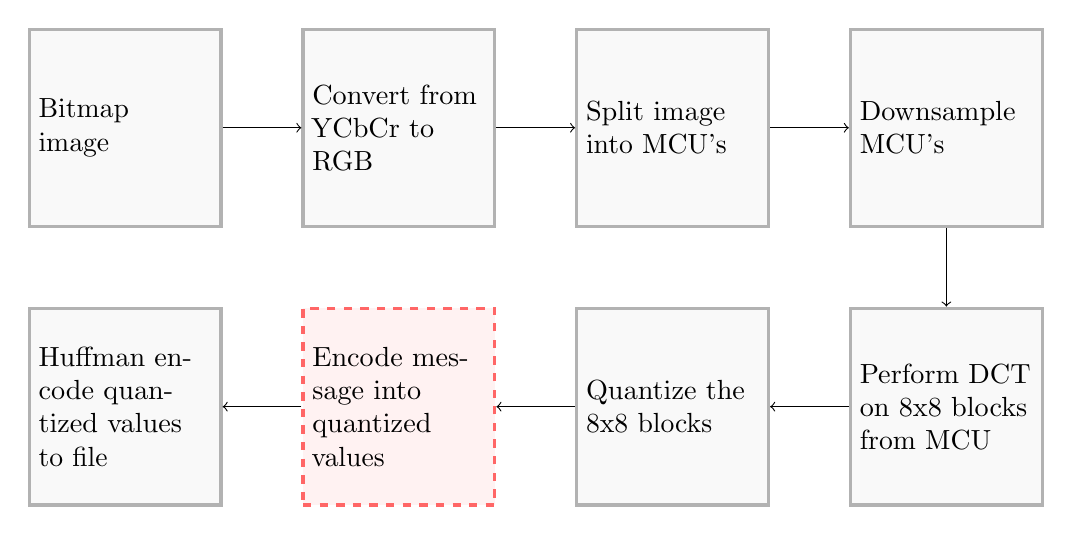
\begin{tikzpicture}[
processnode/.style={rectangle, draw=gray!60, fill=gray!5, very thick, minimum size=5mm,text width=2.2cm, minimum height=2.5cm},
encodenode/.style={rectangle, dashed,draw=red!60, fill=red!5, very thick, minimum size=5mm,text width=2.2cm, minimum height=2.5cm},
pre/.style={=stealth',semithick},
post/.style={->,shorten >=1pt,>=stealth',semithick},
]
%Nodes
\node[processnode]        (huffmanencoding)  {Huffman encode quantized values to file};
\node[encodenode]         (encode)           [right=of huffmanencoding] {Encode message into quantized values};
\node[processnode]        (quantization)     [right=of encode] {Quantize the 8x8 blocks};
\node[processnode]        (dct)              [right=of quantization] {Perform DCT on 8x8 blocks from MCU};
\node[processnode]        (sampling)         [above=of dct] {Downsample MCU's};
\node[processnode]        (split)            [left=of sampling] {Split image into MCU's};
\node[processnode]        (convert)          [left=of split] {Convert from YCbCr to RGB};
\node[processnode]        (bitmapimage)      [left=of convert] {\lstinline|Bitmap| \\image};
 
%Lines
\draw[->] (bitmapimage.east) -- (convert.west);
\draw[->] (convert.east) -- (split.west);
\draw[->] (split.east) -- (sampling.west);
\draw[->] (sampling.south) -- (dct.north);
\draw[->] (dct.west) -- (quantization.east);
\draw[->] (quantization.west) -- (encode.east);
\draw[->] (encode.west) -- (huffmanencoding.east);
\end{tikzpicture}
\caption{Process of encoding a JPEG image with embedding of data}
\label{fig:WrongJPEGprocess}
\end{figure}


\begin{figure}
\centering
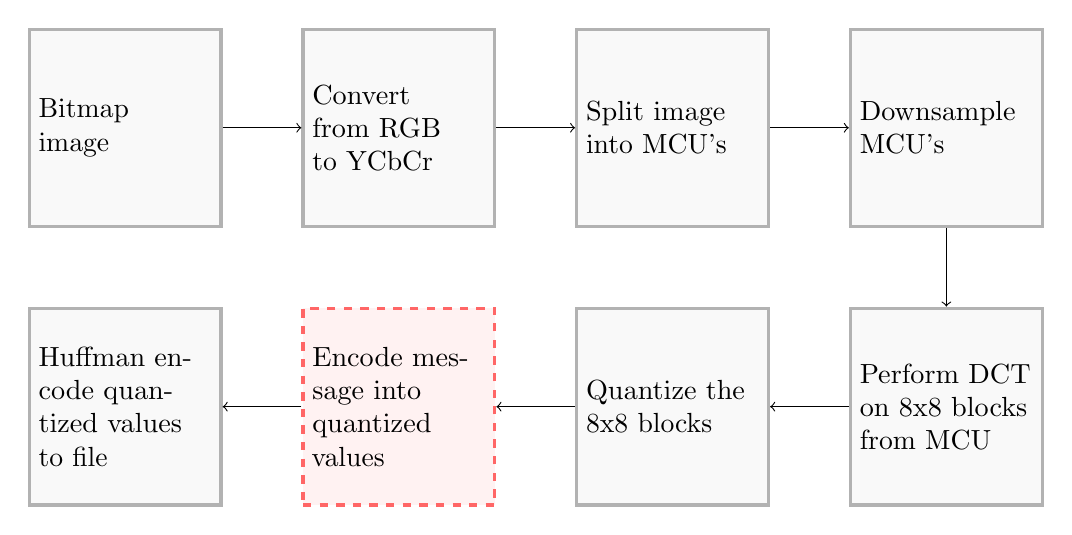
\begin{tikzpicture}[
processnode/.style={rectangle, draw=gray!60, fill=gray!5, very thick, minimum size=5mm,text width=2.2cm, minimum height=2.5cm},
encodenode/.style={rectangle, dashed,draw=red!60, fill=red!5, very thick, minimum size=5mm,text width=2.2cm, minimum height=2.5cm},
pre/.style={=stealth',semithick},
post/.style={->,shorten >=1pt,>=stealth',semithick},
]
%Nodes
\node[processnode]        (huffmanencoding)  {Huffman encode quantized values to file};
\node[encodenode]         (encode)           [right=of huffmanencoding] {Encode message into quantized values};
\node[processnode]        (quantization)     [right=of encode] {Quantize the 8x8 blocks};
\node[processnode]        (dct)              [right=of quantization] {Perform DCT on 8x8 blocks from MCU};
\node[processnode]        (sampling)         [above=of dct] {Downsample MCU's};
\node[processnode]        (split)            [left=of sampling] {Split image into MCU's};
\node[processnode]        (convert)          [left=of split] {Convert from RGB to YCbCr};
\node[processnode]        (bitmapimage)      [left=of convert] {\lstinline|Bitmap| \\image};
 
%Lines
\draw[->] (bitmapimage.east) -- (convert.west);
\draw[->] (convert.east) -- (split.west);
\draw[->] (split.east) -- (sampling.west);
\draw[->] (sampling.south) -- (dct.north);
\draw[->] (dct.west) -- (quantization.east);
\draw[->] (quantization.west) -- (encode.east);
\draw[->] (encode.west) -- (huffmanencoding.east);
\end{tikzpicture}
\caption{Process of encoding a JPEG image with embedding of data}
\label{fig:JPEGprocess}
\end{figure}



\end{document}